\section{Evaluation}

 \frame{\sectionpage}

\begin{frame}{Shock of Surprising Reverses}

    \begin{table}[h!]
        \small
        \begin{center}
          \begin{tabular}{lcc}
            
             & Predicted denial & Predicted success  \\
            \hline
            Actual denial & \uncover<2->{affirm and predicted affirm} & \uncover<2->{affirm but predicted reverse}\\
            Actual success & \uncover<3->{\color{goldenrod}reverse but predicted affirm} & \uncover<2->{reverse and predicted reverse}
          \end{tabular}
        \end{center}
      \end{table}

    \uncover<4->{
        \begin{itemize}
            \item<4-> reverse: denial asylum in the lower court, but grant asylum in the appeal court
            \item<5-> \textbf{\color{goldenrod}surprising reverse}: predicted affirm, but actually reversed
        \end{itemize}
    }
    
\end{frame}

\begin{frame}{Event Study: around Surprising Reverses}

    An event study design around the surprising reverse shock:
    $$
    \bar{y}_{i,s,t}=\alpha D_{s,k} + \beta\mathbf{1}\left(\text{Surprising Reverse}\right)_{s} + \gamma D_{s,k} \times \mathbf{1}\left(\text{Surprising Reverse}\right)_s +\mu_t+ \nu_c+\varepsilon_{i,s,t}
    $$
    where:
    \begin{itemize}
        \item $\bar{y}_{i,s,t}$: the leave-out average grant rate of judge $i$, for case $s$
        \item $\mu_t$: appeal decision year and month fixed effects
        \item $\nu_c$: court fixed effects
        \item $k\in \{T-6,T-5,T-4,T-3,T-2,T-1,T,T+1,T+2,T+3,T+4,T+5,T+6\}$, where $T$ is the time when the appeal decision is made.
    \end{itemize}
     
\end{frame}

\begin{frame}{Event Study: Results}
    \begin{figure}
        \centering
        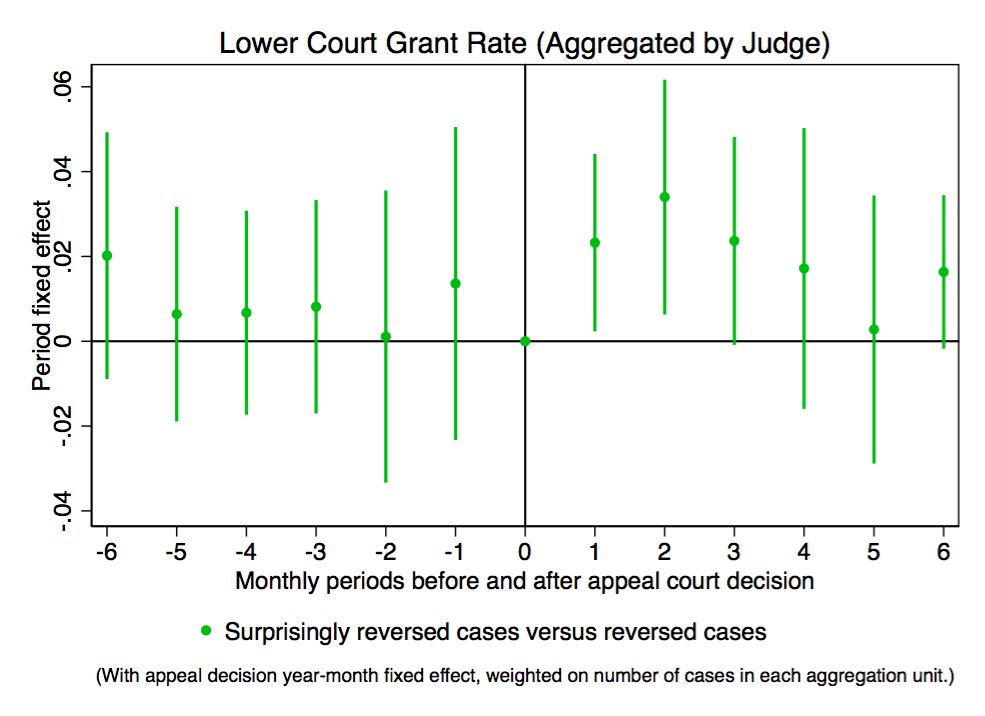
\includegraphics[height = 0.7 \textheight]{images/int_mth1_2.png}
    \end{figure}
    
\end{frame}

\begin{frame}{Event Study: Robustness to Granular Dependent Variable Construction}
    \begin{columns}

        \begin{column}{0.45\textwidth}
            \begin{figure}
            \centering
            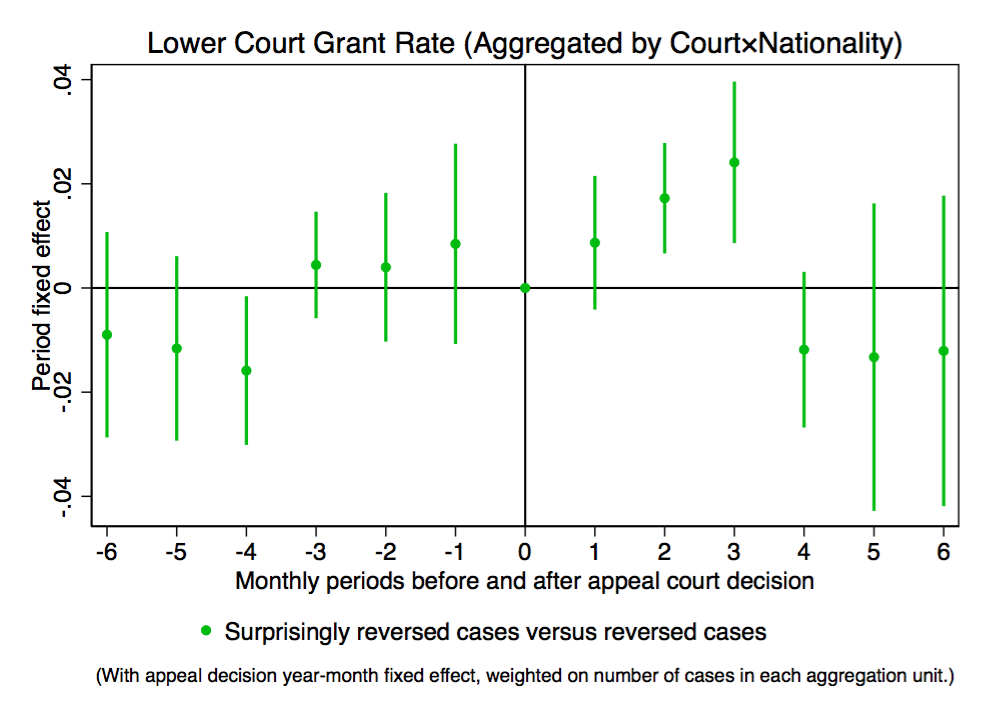
\includegraphics[height = 0.6 \textheight]{images/int_mth3_2.png}
            \end{figure}
        \end{column}
        
        \begin{column}{0.45\textwidth}
            \begin{figure}
                \centering
                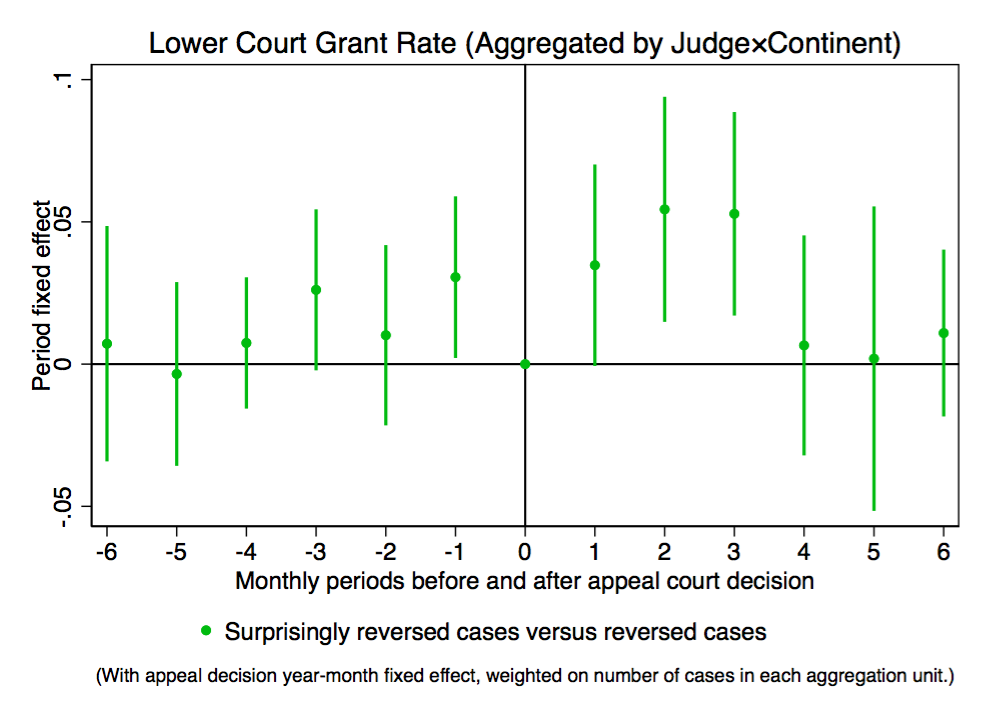
\includegraphics[height = 0.6 \textheight]{images/int_mth4_2.png}
            \end{figure}
        \end{column}
        \end{columns}
    
\end{frame}

\begin{frame}{Event Study: Construct A Measure of Attentiveness}
    \begin{columns}[T]
    \begin{column}{0.5\textwidth}

        \begin{figure}
            \centering
            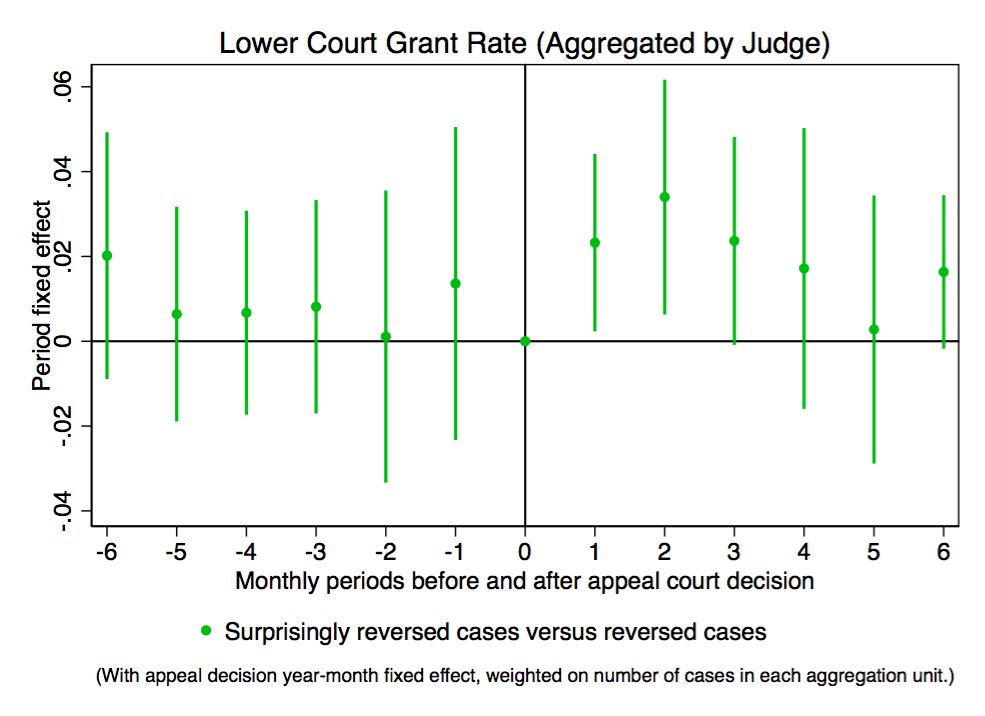
\includegraphics[height = 0.6 \textheight]{images/int_mth1_2.png}
            %\caption{Data Structure}
            \end{figure}
    \end{column}
        
    \begin{column}{0.45\textwidth}
        \small
        \begin{align*}
            \bar{y}_{i,s,t}= &\alpha D_{s,k}\\
            & + \beta\mathbf{1}\left(\text{Surprising Reverse}\right)_{s} \\
            & + \textcolor<3>{goldenrod}{\gamma} D_{s,k} \times \mathbf{1}\left(\text{Surprising Reverse}\right)_s \\
            & +\mu_t+ \nu_c+\varepsilon_{i,s,t}
        \end{align*}
        
        \uncover<2->{Now, limit to a smaller window and re-pool data: $k\in \{T'-1,T',T'+1\}$, and extract $\gamma$ as attentiveness of judges}
    \end{column}
    \end{columns}
    
\end{frame}

\begin{frame}{Validity of the Attentiveness Measure: Judges' Effort}
    \begin{figure}
        \centering
        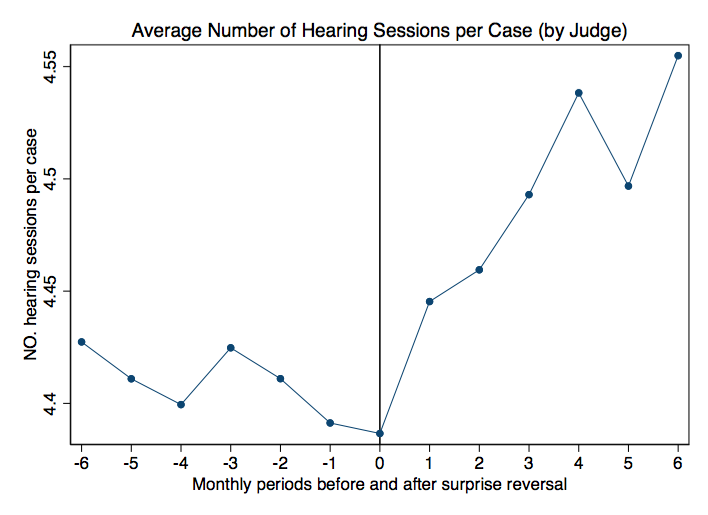
\includegraphics[height = 0.7 \textheight]{images/hearing_num.png}
            %\caption{Data Structure}
    \end{figure}
\end{frame}

\begin{frame}{Validity of the Attentiveness Measure: Judges' Errors}
    \begin{figure}
        \centering
        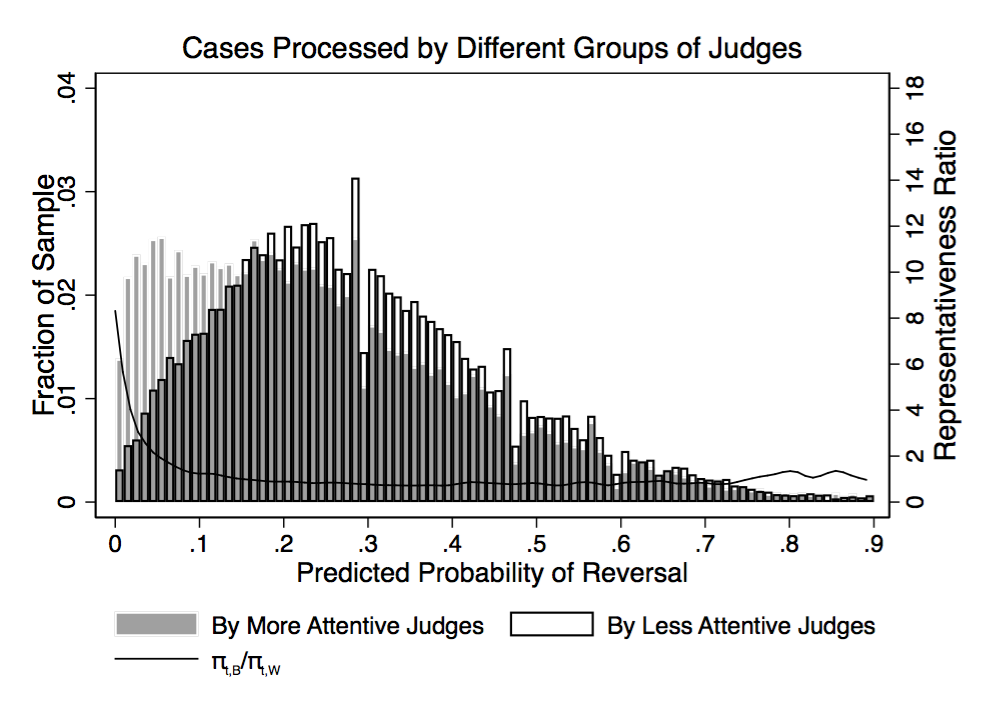
\includegraphics[height = 0.7 \textheight]{images/dist.png}
            %\caption{Data Structure}
    \end{figure}
\end{frame}

\begin{frame}{Validity of the Attentiveness Measure: Early Predictability}
    \begin{columns}

        \begin{column}{0.45\textwidth}
            \begin{figure}
            \centering
            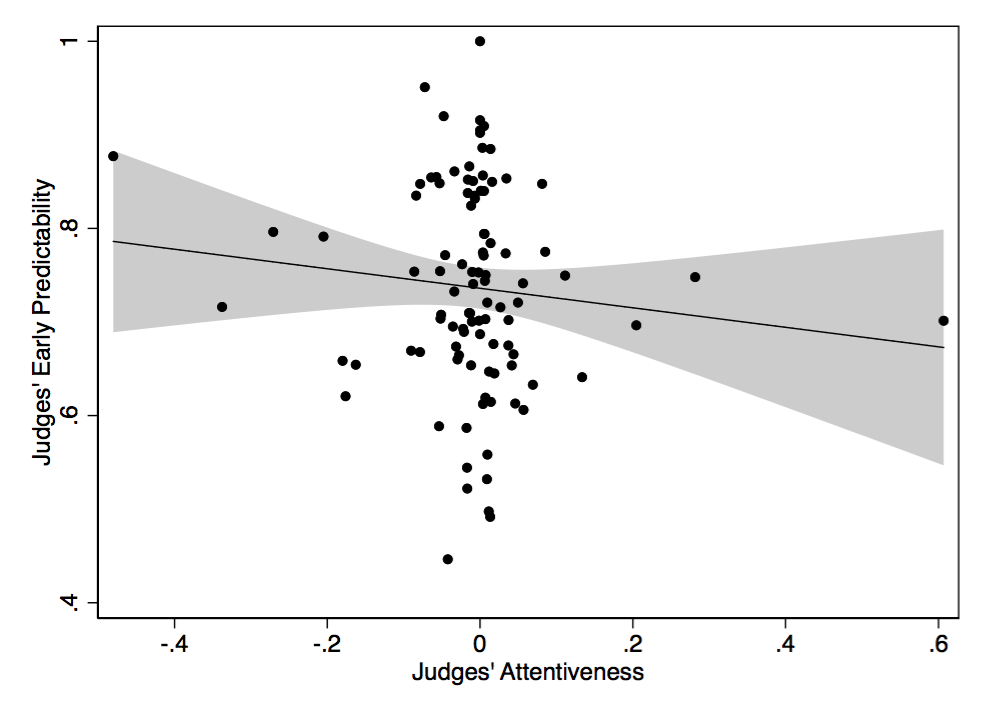
\includegraphics[height = 0.6 \textheight]{images/ep1.png}
            \end{figure}
        \end{column}
        
        \begin{column}{0.45\textwidth}
            \begin{figure}
                \centering
                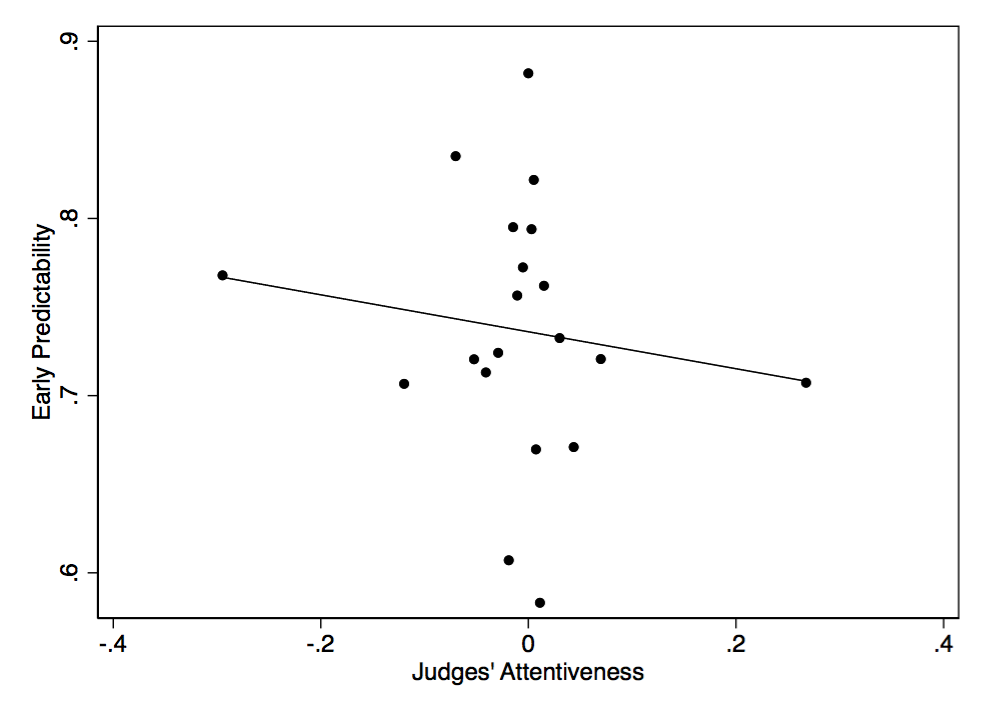
\includegraphics[height = 0.6 \textheight]{images/ep1_bin.png}
            \end{figure}
        \end{column}
        \end{columns}
    
\end{frame}

\begin{frame}{Variation in Attentiveness of Judges}
    \begin{figure}
        \centering
        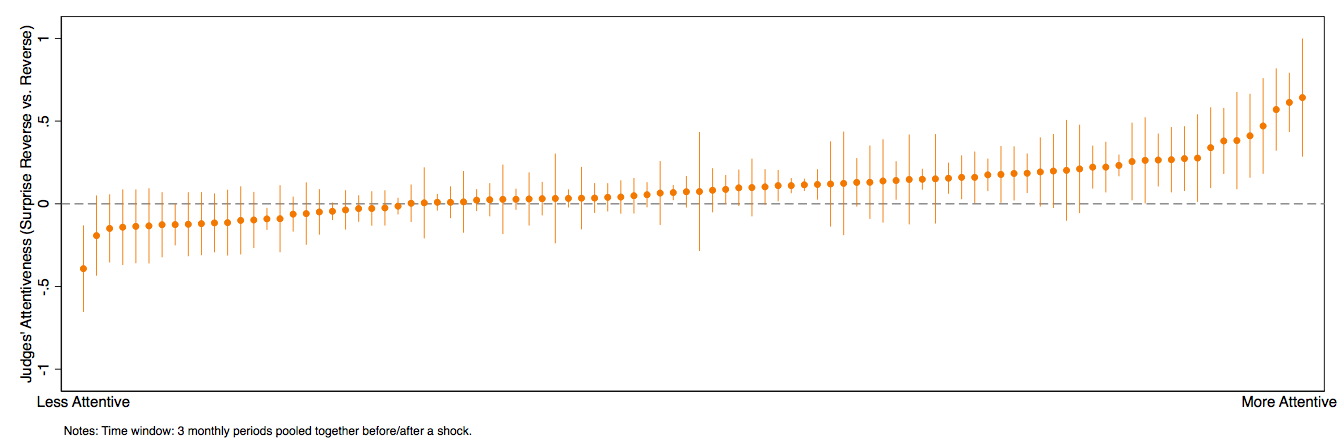
\includegraphics[height = 0.6 \textheight]{images/surp_reverse.png}
        %\caption{Data Structure}
    \end{figure}
\end{frame}

\begin{frame}{The Impact of Judicial Inattention: Implicit Risk Ranking}
    Generate a residualized, leave-out judge leniency measure following \citet{arnold2018racial}:
    \begin{itemize}
        \item<2-> \textbf{\color{goldenrod}\underline{Step 1}}: Regression lower court decisions on court-by-year-by-month FEs
        \item<3-> \textbf{\color{goldenrod}\underline{Step 2}}: Extract the residuals
        \item<4-> \textbf{\color{goldenrod}\underline{Step 3}}: Calculate the leave-out average grant rate in the lower court
    \end{itemize}
    \uncover<5>{
        This will give us a leniency measure
    }
\end{frame}

\begin{frame}{Risk Ranking of Judges}
    \begin{figure}
        \centering
        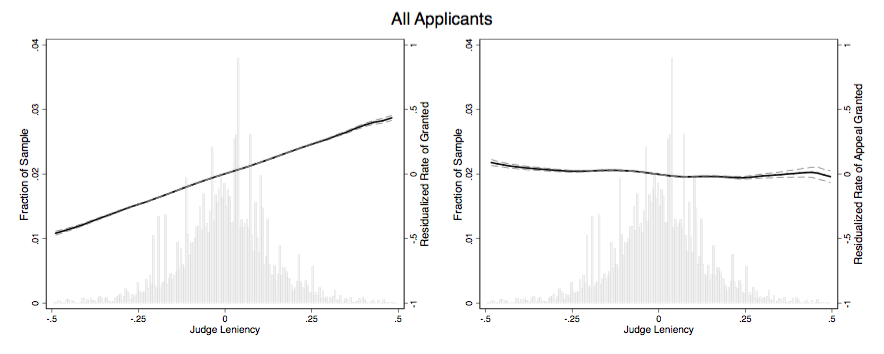
\includegraphics[height = 0.7 \textheight]{images/complete_full.png}
        %\caption{Data Structure}
    \end{figure}
\end{frame}

\begin{frame}{Risk Ranking of Judges: Appeal Courts}
    \begin{figure}
        \centering
        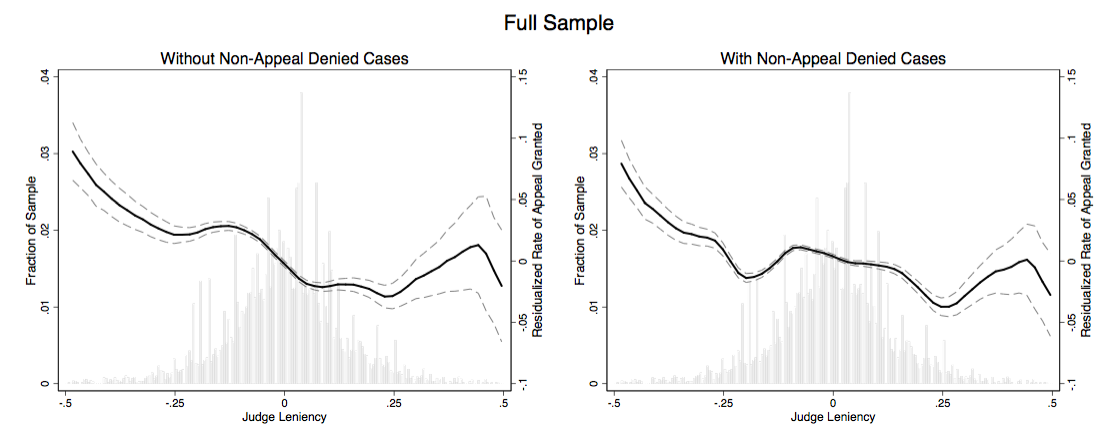
\includegraphics[height = 0.7 \textheight]{images/stage2comp_full.png}
        %\caption{Data Structure}
    \end{figure}
\end{frame}

\begin{frame}{Implicit Risk Ranking and Inattention}
    \begin{figure}
        \centering
        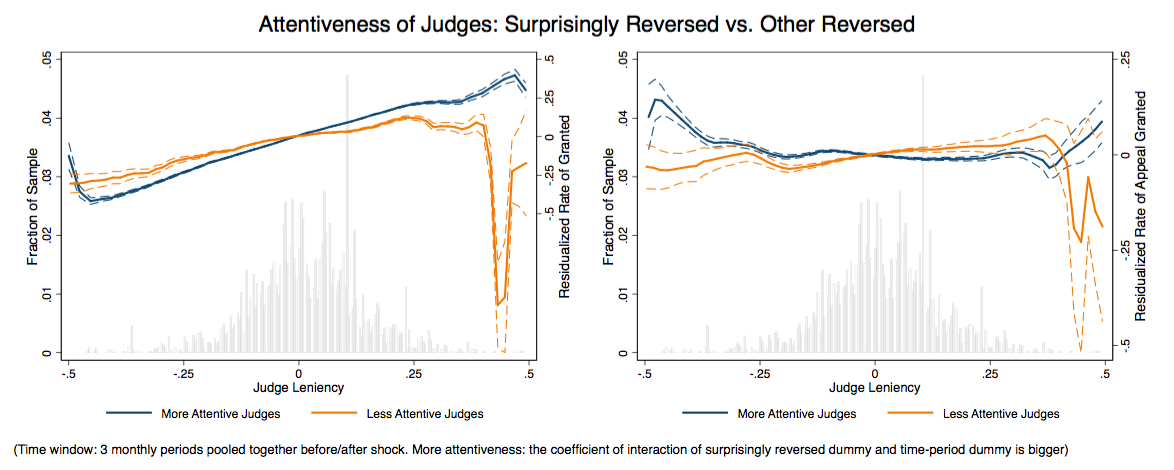
\includegraphics[height = 0.7 \textheight]{images/complete_surp_inattent.png}
        %\caption{Data Structure}
    \end{figure}
    
\end{frame}

\begin{frame}{Risk Ranking of Judges: Asian Applicants}
    \begin{figure}
        \centering
        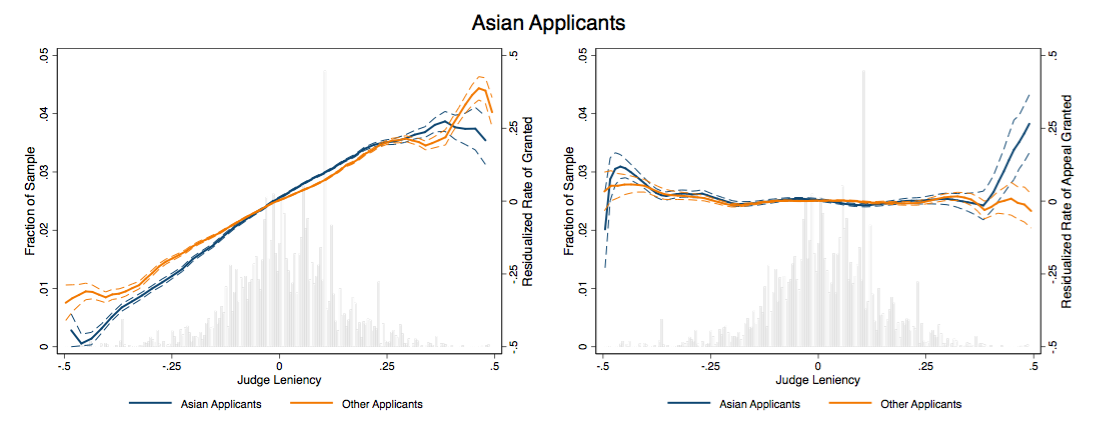
\includegraphics[height = 0.7 \textheight]{images/comp_asia.png}
        %\caption{Data Structure}
    \end{figure}
\end{frame}

\begin{frame}{Risk Ranking of Judges: Government Experience}
    \begin{figure}
        \centering
        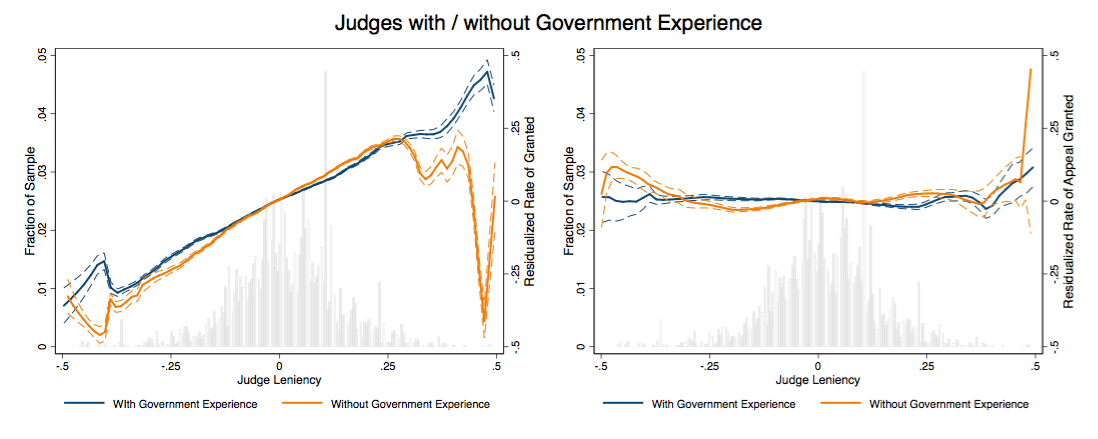
\includegraphics[height = 0.7 \textheight]{images/comp_govt_dum.png}
        %\caption{Data Structure}
    \end{figure}
\end{frame}

\begin{frame}{Risk Ranking of Judges: Workload}
    \begin{figure}
        \centering
        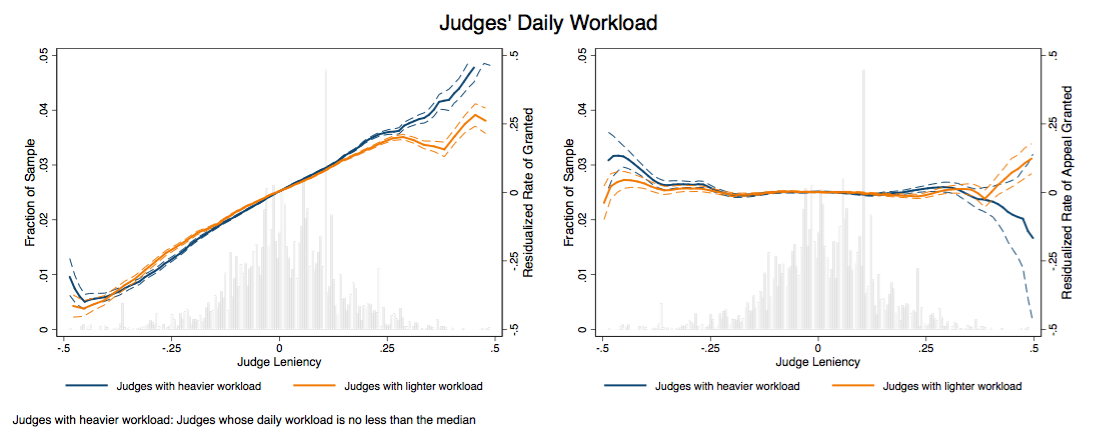
\includegraphics[height = 0.7 \textheight]{images/comp_judge_morecase_perday.png}
        %\caption{Data Structure}
    \end{figure}
\end{frame}

\begin{frame}{Judges' Inattention: Experience Heterogeneity}
    \begin{figure}
        \centering
        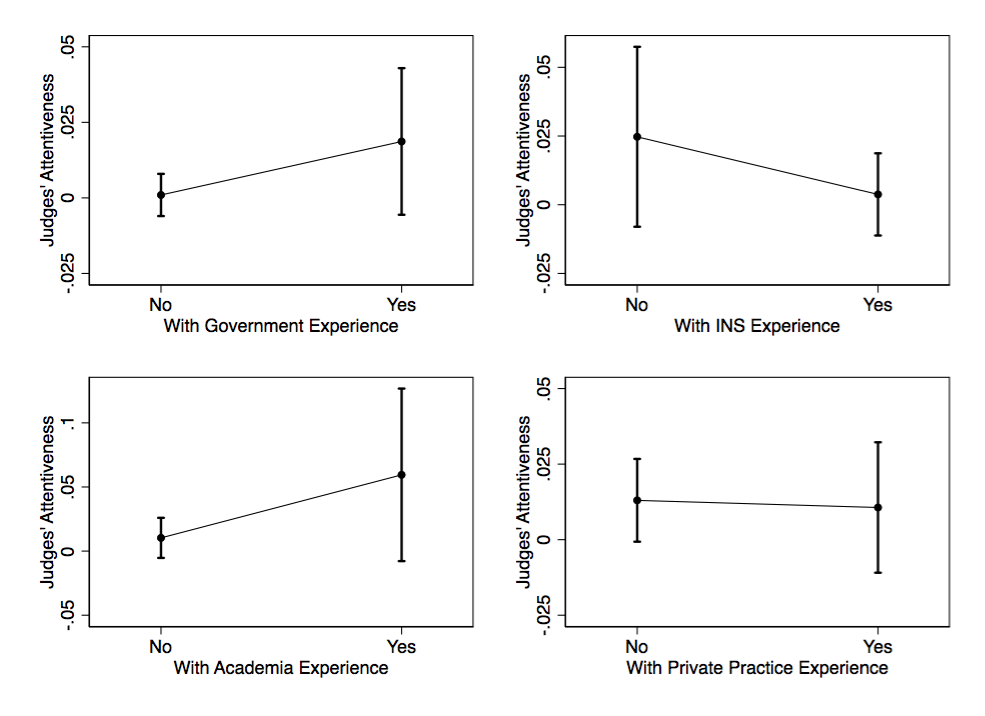
\includegraphics[height = 0.8 \textheight]{images/judge_expdum_full.png}
            %\caption{Data Structure}
    \end{figure}
\end{frame}

\begin{frame}{Judges' Inattention: Experience Heterogeneity}
    \begin{figure}
        \centering
        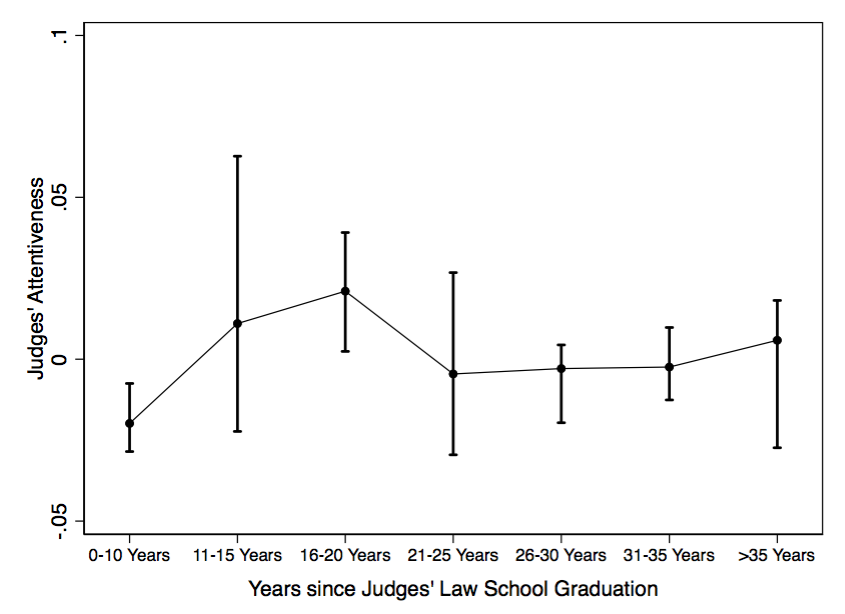
\includegraphics[height = 0.6 \textheight]{images/attent_bylschyr_mean.png}
            %\caption{Data Structure}
    \end{figure}
\end{frame}

\begin{frame}{Judges' Inattention: Gender Heterogeneity}
    \begin{figure}
        \centering
        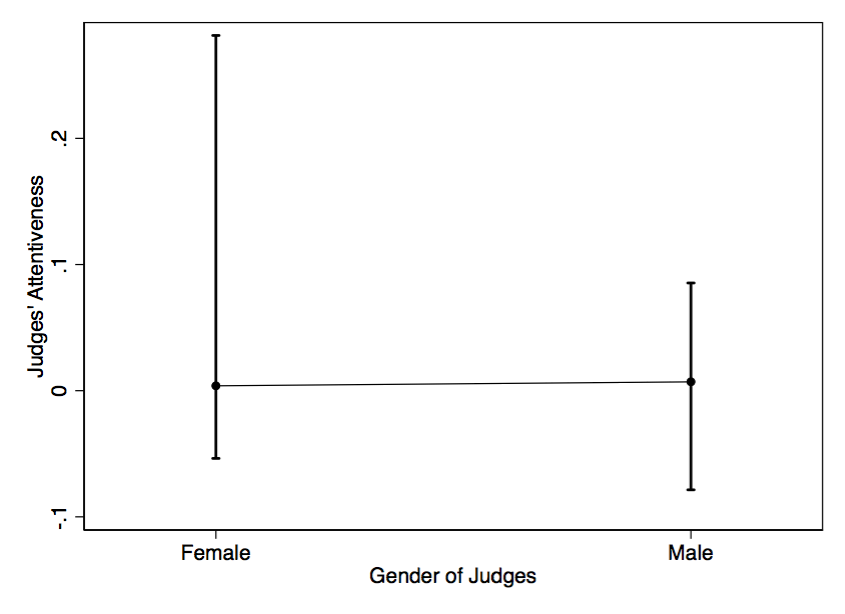
\includegraphics[height = 0.6 \textheight]{images/attent_bygender.png}
            %\caption{Data Structure}
    \end{figure}
\end{frame}

